\documentclass[../main/main.tex]{subfiles}

\newdate{date}{28}{09}{2020}

% \begin{figure}[h!]
% \centering
% \includegraphics[page=6,width=0.8\textwidth]{../lessons/pdf_file/03_lecture.pdf}
% \end{figure}

%\displaydate{date}. Compiled:  \today. Alice.

\begin{document}

\pagestyle{plain}

\section{Lecture 3}


\subsubsection*{Slide 1}

\begin{minipage}[]{0.5\linewidth}
\centering
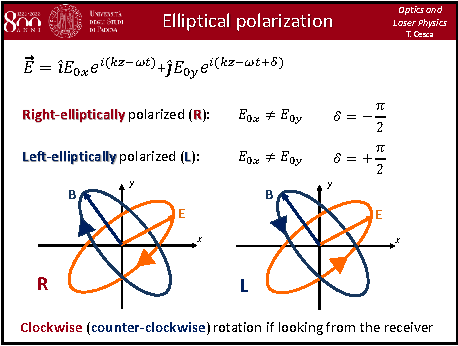
\includegraphics[page=1,width=1\textwidth]{../lessons/pdf_file/03_lecture.pdf}
\end{minipage}
\hspace{0.3cm}\vspace{0.3cm}
\begin{minipage}[c]{0.47\linewidth}

In ther last lecture we have seen how to obtain elleiptical polarization. If we have a left-elleptically polarized way we have a counter-clock-wise rotation, while for right-elliptically we have a clowise rotation.

How can we physically get the overlap of two components with a given phase shift in order to get an elliptical polarization?

\end{minipage}

\subsubsection*{Slide 2}

\begin{minipage}[]{0.5\linewidth}
\centering
\includegraphics[page=2,width=1\textwidth]{../lessons/pdf_file/03_lecture.pdf}
\end{minipage}
\hspace{0.3cm}\vspace{0.3cm}
\begin{minipage}[c]{0.47\linewidth}

To do this, we have to make a step back and say few things about the propagation on crystals. In general, we think that is always possible to cut such crystal in such a way that you have for any given direction of propagation vector two possible refractive index (which means two possible velocities) corresponding to orthogonal polarization state. In particular you get \textbf{birefringence}. So the idea is that you can always cut a crystal such that you have two possible refractive indexes.

The \textbf{optic axis} is the direction for which you have the same refractive indexes.


\end{minipage}

\subsubsection*{Slide 3}

\begin{minipage}[]{0.5\linewidth}
\centering
\includegraphics[page=3,width=1\textwidth]{../lessons/pdf_file/03_lecture.pdf}
\end{minipage}
\hspace{0.3cm}\vspace{0.3cm}
\begin{minipage}[c]{0.47\linewidth}

You can distinguish three classes of crystals.
\begin{itemize}
\item \textbf{isotropic}: there is no birefringence for any propagation direction. We have only one refractive index.

\item \textbf{uniaxial}: this family of crystals have one optic axis. We have two different refractive indexes associated to orthogonal polarizations. The \textbf{ordinary waves} are electromagnetic waves linearly polarized perpendicularly to the optic axis and to the propagation direction. The \textbf{extraordinary waves} for those field parallel to the optic axis and perdpendicular to the propagation direction.

\item \textbf{biaxial}: we have two different optics axis, such that we can have 3 different refractive indexes for the 3 different orientation.

\end{itemize}
\end{minipage}

\newpage

\subsubsection*{Slide 4}

\begin{minipage}[]{0.5\linewidth}
\centering
\includegraphics[page=4,width=1\textwidth]{../lessons/pdf_file/03_lecture.pdf}
\end{minipage}
\hspace{0.3cm}\vspace{0.3cm}
\begin{minipage}[c]{0.47\linewidth}

In order to answer to the question: how can we physically get the overlap of two components with a given phase shift in order to get an elliptical polarization?
We will consider \textbf{uniaxial crystals}. We can distinguish two families:
\begin{itemize}
\item \textbf{positive}: the extraordinary refractive index is larger than the ordinary.

\item \textbf{negative}: the contrary of positive.

\end{itemize}

Here, is reported a table of differen uniaxial crystals. The most used one is \emph{calcite}.

How can we use birefringence to control the polarization state of our wave?

\end{minipage}

\subsubsection*{Slide 5}

\begin{minipage}[]{0.5\linewidth}
\centering
\includegraphics[page=5,width=1\textwidth]{../lessons/pdf_file/03_lecture.pdf}
\end{minipage}
\hspace{0.3cm}\vspace{0.3cm}
\begin{minipage}[c]{0.47\linewidth}

Let us suppose that now we have a material with two different refractive indexes related to orthogonal polarization space. We can imagine to align our system of reference in order to have an \( x \) axis related to one refractive index and a \( y \) axis related to the other. When wave propagates trough a crystal aligned in this way, we can introduce a \textbf{phase shift} due to the difference of optical path. If you cut the material with the thickness in such a way that we have \( \Delta \Phi = \pi /2 \), we have that:
\begin{equation*}
  d (n_y - n_x) = \lambda /4
\end{equation*}
so we are realizing a \textbf{quarter wave plate}.
In this way, we will get an elliptical polarization. The \( x \) axis is the \textbf{fast axis} (the wave velocity is faster).
If the \textbf{fast} axis is vertical (instead of being orizontal) we obtain \( \Delta \Phi = - \pi /2 \). So the sign depends on where is oriented the fast axis.

\end{minipage}

\subsubsection*{Slide 6}

\begin{minipage}[]{0.5\linewidth}
\centering
\includegraphics[page=6,width=1\textwidth]{../lessons/pdf_file/03_lecture.pdf}
\end{minipage}
\hspace{0.3cm}\vspace{0.3cm}
\begin{minipage}[c]{0.47\linewidth}

This can be used to obtain also a circular polarization. If you start with a linear polarization state and if you orient the transmission axis to \( 45° \) with respect to the fast axis, you will obtain \( E_{0x}=E_{0y} \).

\end{minipage}

\newpage

\subsubsection*{Slide 7}

\begin{minipage}[]{0.5\linewidth}
\centering
\includegraphics[page=7,width=1\textwidth]{../lessons/pdf_file/03_lecture.pdf}
\end{minipage}
\hspace{0.3cm}\vspace{0.3cm}
\begin{minipage}[c]{0.47\linewidth}
With the same idea, you can also realize \textbf{Half waveplate}. You select the thickness of your material in such a way to obtain \( \Delta \Phi = \pi  \).

This is the expression of the elctric fiedl after passing trough this material, you have to sum up two components with a phase of \( \pi  \). If we remember that \( e^{\pm i \pi } = -1 \), we are just flipping the component and we obtain a rotation. If we incide with a linear polarized wave with angle \( \alpha  \), we will get still a linearly polarized wave but rotating by \( 2 \alpha  \). This is the same both if you introduce a phase shift of \( \pi  \) or \( -\pi  \). So in this case does not matter what you are orienting along the orizontal axis. In any case you will have a rotation.
This is useful if you want to obtain a rotation of 90° which you cannot obtain with a linear polarization (you cannot obtain this with a linear polarizer as we have already seen in the last lectures!).

\end{minipage}

\subsubsection*{Slide 8}

\begin{minipage}[]{0.5\linewidth}
\centering
\includegraphics[page=8,width=1\textwidth]{../lessons/pdf_file/03_lecture.pdf}
\end{minipage}
\hspace{0.3cm}\vspace{0.3cm}
\begin{minipage}[c]{0.47\linewidth}

\textbf{Jones' notation} is a very useful notation for polarized waves. Let us consider a wave and decompose it into two direction with a phase shift contained in the \( y \) direction (\( \delta  \)).

We can write this in a more compact wave if we introduce \( \va{E}_0 \).
If the two components are both real we are talking about \textbf{linear polarization}, while if they are complex we are dealing with an \textbf{elliptic polarization} state.
We have a \textbf{circular polarization} if the modulus are the same.

With this idea in mind, we introduce a \textbf{Jones' vector}, which is simply a vector which contain the two components. We can have also its normalized form.


\end{minipage}

\subsubsection*{Slide 9}

\begin{minipage}[]{0.5\linewidth}
\centering
\includegraphics[page=9,width=1\textwidth]{../lessons/pdf_file/03_lecture.pdf}
\end{minipage}
\hspace{0.3cm}\vspace{0.3cm}
\begin{minipage}[c]{0.47\linewidth}

In this way, we can immeadialy write a Jones' vector for a linearly polarized way and so on.



\end{minipage}

\subsubsection*{Slide 10}

\begin{minipage}[]{0.5\linewidth}
\centering
\includegraphics[page=10,width=1\textwidth]{../lessons/pdf_file/03_lecture.pdf}
\end{minipage}
\hspace{0.3cm}\vspace{0.3cm}
\begin{minipage}[c]{0.47\linewidth}
If we combine the left and right circularly polarized way we apply the Jones'notation and we sum the two components. We obtain a Jones'vector for a linearly polarized wave.

\end{minipage}

\subsubsection*{Slide 11}

\begin{minipage}[]{0.5\linewidth}
\centering
\includegraphics[page=11,width=1\textwidth]{../lessons/pdf_file/03_lecture.pdf}
\end{minipage}
\hspace{0.3cm}\vspace{0.3cm}
\begin{minipage}[c]{0.47\linewidth}

Jones'notation is useful particularly because you can also associate to any optical element which produce an effect on the polarization state you can introduce a \textbf{Jones'matrix}.

By simply applying in sequence all the matrices of the different optical elements to specific order to the incidence polarization state, you will have the final polarization state of your wave. Pay attention to the order of applications of the operators!

\end{minipage}

\subsubsection*{Slide 12}

\begin{minipage}[]{0.5\linewidth}
\centering
\includegraphics[page=12,width=1\textwidth]{../lessons/pdf_file/03_lecture.pdf}
\end{minipage}
\hspace{0.3cm}\vspace{0.3cm}
\begin{minipage}[c]{0.47\linewidth}

In this slide there is a summary of the main Jones'matrices for the different optical elements.


\end{minipage}

\subsubsection*{Slide 13}

\begin{minipage}[]{0.5\linewidth}
\centering
\includegraphics[page=13,width=1\textwidth]{../lessons/pdf_file/03_lecture.pdf}
\end{minipage}
\hspace{0.3cm}\vspace{0.3cm}
\begin{minipage}[c]{0.47\linewidth}

Let us try to apply the Jones'notation. Let us see this excercise. We have just seen the result in this lecture.

We have a linearly polarized wave at \( 45° \) degrees. We apply QWP Jones'matrix.


\end{minipage}

\subsubsection*{Slide 14}

\begin{minipage}[]{0.5\linewidth}
\centering
\includegraphics[page=14,width=1\textwidth]{../lessons/pdf_file/03_lecture.pdf}
\end{minipage}
\hspace{0.3cm}\vspace{0.3cm}
\begin{minipage}[c]{0.47\linewidth}

THis is the graphical answer to the exercise as we have already seen.

\end{minipage}

\subsubsection*{Slide 15}

\begin{minipage}[]{0.5\linewidth}
\centering
\includegraphics[page=15,width=1\textwidth]{../lessons/pdf_file/03_lecture.pdf}
\end{minipage}
\hspace{0.3cm}\vspace{0.3cm}
\begin{minipage}[c]{0.47\linewidth}

An important point is that \textbf{there is no Jones'vector for describing unpolarized ligth!} The vector \( \begin{pmatrix}
0 \\
0
\end{pmatrix}  \) does not mean unpolarized ligth! Instead this means that there is no ligth coming out, does not mean an unpolarized state.


\end{minipage}

\subsubsection*{Slide 16}

\begin{minipage}[]{0.5\linewidth}
\centering
\includegraphics[page=16,width=1\textwidth]{../lessons/pdf_file/03_lecture.pdf}
\end{minipage}
\hspace{0.3cm}\vspace{0.3cm}
\begin{minipage}[c]{0.47\linewidth}

Let us try to solve this exercise with this notation. Let us consider an incident unpolarized ligth, which imping on a linear polarizer of 45°. We have then a QWP with vertical fast axis, another QWP with vertical fast axis and finally a linear polarizer of 45° degrees.
What is coming out at the end?

With an unpolarized ligth which passed trough a linear polarizer at \( 45° \), we obtain a linear polarized wave at 45°. If then we enter on a QWP, we obtain a circularly polarized wave right (the fast axis is vertical). Then, if we enter again on a QWP we obtain polarized ligth at -45°. \textbf{The two QWP in sequence work as one HWP}. If we enter with a light with a -45° degree on a polarizer at 45° the result is zero. There is no ligth coming out.

\end{minipage}

\subsubsection*{Slide 17}

\begin{minipage}[]{0.5\linewidth}
\centering
\includegraphics[page=17,width=1\textwidth]{../lessons/pdf_file/03_lecture.pdf}
\end{minipage}
\hspace{0.3cm}\vspace{0.3cm}
\begin{minipage}[c]{0.47\linewidth}

Another interesting exercise is to answer to the question: whar are the polarizations state which pass uneffected trough the opritcal elements represented by such Jones'matrix?
We are solving an eigenvectors and eigenvalue problem for a given optical element or for a sequence of them.
We obtain two eigenvalues.

The eigenvectors are the polarization states which pass uneffected trough the sequence of optical elements.

\end{minipage}

\subsubsection*{Slide 18}

\begin{minipage}[]{0.5\linewidth}
\centering
\includegraphics[page=18,width=1\textwidth]{../lessons/pdf_file/03_lecture.pdf}
\end{minipage}
\hspace{0.3cm}\vspace{0.3cm}
\begin{minipage}[c]{0.47\linewidth}

For instance, let us determine the eigenvectors of a QWP with horizontal fast axis.
The ratio of the two eigenvalues is \( i \), so the two eigenvectors have a phase shift of \( \pi /2 \) which is what we get for QWP.

The important idea of Jones'notatio is that you can determine the final polarization state (or an intermediate one) by computing matrix-product.


\end{minipage}



\end{document}
